\documentclass[10pt, aspectratio=169, handout]{beamer}
\usefonttheme{professionalfonts}

\mode<presentation>
{
  \usetheme{Berkeley}
  \usecolortheme{beaver}
  \usefonttheme{default}
  \setbeamertemplate{navigation symbols}{}
  \setbeamertemplate{caption}[numbered]
} 

\setbeamertemplate{footline}{%
  \leavevmode%
  \hbox{%
    \begin{beamercolorbox}[wd=.85\paperwidth,ht=2.5ex,dp=1ex,left]{author in head/foot}%
      \usebeamerfont{author in head/foot}Maxx Seminario, Electronic Circuits, Spring 2026%
    \end{beamercolorbox}%
    \begin{beamercolorbox}[wd=.15\paperwidth,ht=2.5ex,dp=1ex,right]{date in head/foot}%
      \hspace*{0.5em}\insertframenumber{} / \inserttotalframenumber\hspace*{0.5em}%
    \end{beamercolorbox}%
  }%
  \vskip0pt%
}

\usepackage[english]{babel}
\usepackage[utf8]{inputenc}
\usepackage{tikz}
\usepackage{pgfplots}
\usepackage{array}
\usepackage{makecell}
\usepackage{verbatim}
\usepackage{graphicx}
\usepackage{subcaption}
\usepackage{amsfonts}
\usepackage{amsmath}
\usepackage{bm}
\usepackage{epstopdf}
\usepackage[american]{circuitikz}
\usepackage{caption}
\captionsetup{compatibility=false}
\usepackage[absolute,overlay]{textpos}
\usetikzlibrary{calc}
\usetikzlibrary{pgfplots.fillbetween, backgrounds}
\usetikzlibrary{positioning}
\usetikzlibrary{pgfplots.groupplots}
\usetikzlibrary{plotmarks}
\usetikzlibrary{calc}
\usetikzlibrary{decorations.markings}
\usetikzlibrary{arrows.meta,calc}

\usepgfplotslibrary{groupplots}
\pgfplotsset{compat=newest} 

\usepackage{hyperref}
\hypersetup{
    colorlinks=true,
    linkcolor=blue,
    filecolor=magenta,      
    urlcolor=cyan,
}

% Added by Maxx Seminario 01/06/2026 - for colored icons in itemize labels
\usepackage{wasysym} % for smiles and frowns
\newcommand{\neutralface}{%
  \tikz[baseline=-0.6ex]{
    \draw (0,0) circle (0.9ex);
    \fill (-0.35ex,0.25ex) circle (0.12ex);
    \fill ( 0.35ex,0.25ex) circle (0.12ex);
    \draw (-0.35ex,-0.25ex) -- (0.35ex,-0.25ex);
  }%
}
\newcommand{\baditem}{\textcolor{red!70!black}{\frownie}}
\newcommand{\gooditem}{\textcolor{green!60!black}{\smiley}}
\newcommand{\mehitem}{\textcolor{orange!80!black}{\neutralface}}

\title[ECEN 222]{Introduction to Diodes}
\author{Maxx Seminario}
\institute{University of Nebraska-Lincoln}
\date{Spring 2026}

\begin{document}
\begin{frame}
  \titlepage
\end{frame}

\section{Introduction}

\begin{frame}{What is a Diode?}
    
    \begin{columns}[t]
    \column{0.48\textwidth}
        \textbf{The Basic Idea}:
        \begin{itemize}
            \item Two-terminal semiconductor device
            \item Conducts current in one direction
            \item Blocks current in the other direction
        \end{itemize}
        
        % \vspace{0.5em}
        \textbf{Symbol and Terminals}:
        
        \begin{center}
        \begin{circuitikz}[scale=1.5]
            \draw (0,0) to[D, l=$D$, v=$v_D$, i=$i_D$] (3,0);
            \node[below] at (0,-0.3) {Anode (+)};
            \node[below] at (3,-0.3) {Cathode (-)};
            \draw[->, red, thick] (1.0,0.7) -- (2.0,0.7);
            \node[red] at (1.5,0.9) {Current flow};
        \end{circuitikz}
        \end{center}
        
        \vspace{-0.3cm}
        Triangle points in direction of current flow
    
    \column{0.48\textwidth}
        \textbf{Physical Device}:
        
        \begin{center}
        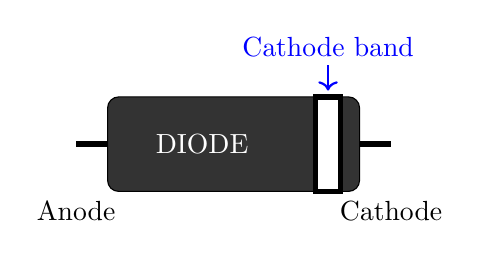
\begin{tikzpicture}[scale=0.8]
            % Diode body
            \draw[fill=black!80, rounded corners] (0,0) rectangle (4,1.5);
            
            % Cathode band
            \draw[fill=white, line width=2pt] (3.3,0) rectangle (3.7,1.5);
            
            % Leads
            \draw[line width=2pt] (-0.5,0.75) -- (0,0.75);
            \draw[line width=2pt] (4,0.75) -- (4.5,0.75);
            
            % Labels
            \node[white] at (1.5,0.75) {DIODE};
            \node[below] at (-0.5,0) {Anode};
            \node[below] at (4.5,0) {Cathode};
            \draw[->, blue, thick] (3.5,2) -- (3.5,1.6);
            \node[blue] at (3.5,2.3) {Cathode band};
        \end{tikzpicture}
        \end{center}
        
        \vspace{-0.2cm}
        \textbf{Key Applications}:
        \begin{itemize}
            \item Rectification (AC to DC)
            \item Voltage regulation
            \item Signal clipping and protection
            \item Logic circuits
        \end{itemize}
    
    \end{columns}
    
\end{frame}

\section{Diode I-V Characteristics}

\begin{frame}{The Shockley Diode Equation}
    
    The relationship between voltage and current in a diode is described by the \textbf{Shockley equation}: 

    \vspace{-0.6cm}
    
    \begin{equation*}
        i_D = I_S \left( e^{v_D / n V_T} - 1 \right)
    \end{equation*}
    
    \vspace{-0.15cm}
    
    \begin{columns}[t]
    \column{0.48\textwidth}
        \textbf{Parameters}:
        \begin{itemize}
            \item $i_D$ = diode current
            \item $v_D$ = voltage across diode
            \item $I_S$ = saturation current ($\approx 10^{-14}$ A)
            \item $n$ = ideality factor (1-2)
            \item $V_T$ = $kT/q$ = thermal voltage  \\ 
            (about 25 mV at room temperature)
            \item $k$ = Boltzmann's constant
            \item $T$ = absolute temperature (K)
            \item $q$ = elementary charge
        \end{itemize}
    
    \column{0.48\textwidth}
        \textbf{Exponential Behavior}:
        
        \begin{center}
        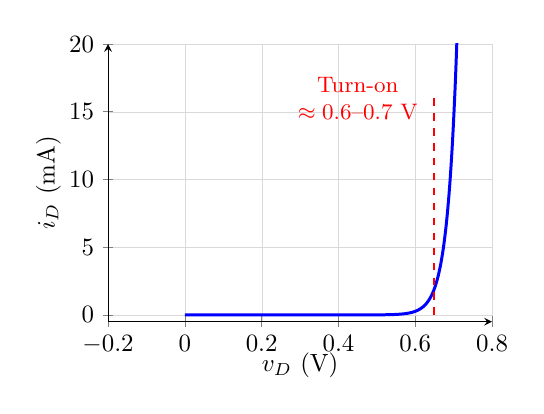
\begin{tikzpicture}[scale=0.9]
            \begin{axis}[
                width=7cm, 
                height=5.5cm,
                xlabel={$v_D$ (V)},
                ylabel={$i_D$ (mA)},
                xmin=-0.2, 
                xmax=0.8,
                ymin=-0.5, 
                ymax=20,
                grid=major,
                grid style={line width=0.1pt, draw=gray!30},
                axis lines=left,
                every axis x label/.style={at={(axis description cs: 0.5,-0.08)}, anchor=north},
                every axis y label/.style={at={(axis description cs:-0.1,0.5)}, rotate=90, anchor=south},
            ]
            
            % Forward characteristic using Shockley equation
            % i_D = I_S * (exp(v_D / (n*V_T)) - 1)
            % Scaled for mA output with I_S=1e-14, n=1, V_T=0.025
            \addplot[
                blue, 
                very thick,
                smooth,
                domain=0:0.75,
                samples=100
            ] {1e-11 * (exp(x/0.025) - 1)};
            
            % Highlight knee region
            \draw[red, dashed, thick] (axis cs: 0.65,0) -- (axis cs:0.65,16);
            \node[red, align=center, font=\small] at (axis cs:0.45,16) {Turn-on \\ $\approx 0.6$--$0.7$ V};
            
            \end{axis}
        \end{tikzpicture}
        \end{center}
        
        \vspace{-0.5cm}

        Current increases exponentially with voltage
        
    \end{columns}
    
\end{frame}

\begin{frame}{Forward Bias Operation}
    
    \textbf{Forward Bias}:  Positive voltage applied to anode relative to cathode ($v_D > 0$)
    
    \vspace{0.5em}
    
    \begin{columns}[t]
    \column{0.6\textwidth}
        \textbf{Behavior}:
        \begin{itemize}
            \item Little current until $v_D \approx 0.5$--$0.6$ V
            \item Current increases rapidly above this
            \item $v_D \approx 0.7$ V when conducting
            \item Voltage stays about constant once "on"
        \end{itemize}
        
        \begin{center}
       \begin{circuitikz}[scale=0.8]
            % Actual diode
            \draw (0,2) to[V, l_=$V_S$] (0,0)
                to[short] (2.5,0)
                to[D, l=$D$] (2.5,2)
                to[R, l=$R$] (0,2);
            \node at (1.25,-0.5) {Actual diode};
            
            % Simplified model
        \draw (5,2) to[V, l_=$V_S$] (5,0)
            to[short] (7.5,0)
            to[battery1, l=$0.7$ V, invert] (7.5,2)
            to[R, l=$R$] (5,2);
        \node at (6.25,-0.5) {Simplified model};
        \end{circuitikz}
        \end{center}
        
    \column{0.4\textwidth}
        \textbf{I-V Characteristic}:
        
        \begin{center}
        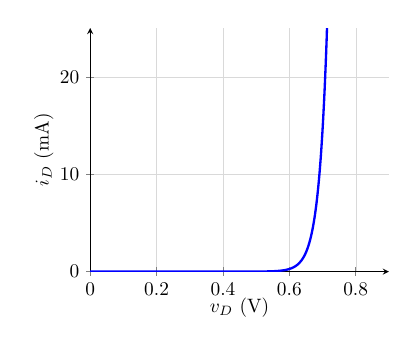
\begin{tikzpicture}[scale=0.7]
            \begin{axis}[
                width=7cm, 
                height=6cm,
                xlabel={$v_D$ (V)},
                ylabel={$i_D$ (mA)},
                xmin=0, 
                xmax=0.9,
                ymin=0, 
                ymax=25,
                grid=major,
                grid style={line width=0.1pt, draw=gray!30},
                axis lines=left,
                every axis x label/.style={at={(axis description cs:0.5,-0.08)}, anchor=north},
                every axis y label/.style={at={(axis description cs:-0.1,0.5)}, rotate=90, anchor=south},
            ]
            
            % Forward characteristic using Shockley equation
            % Using restrict y to prevent dimension overflow
            \addplot[
                blue, 
                very thick,
                smooth,
                domain=0:0.87,
                samples=150,
                restrict y to domain=0:30
            ] {min(1e-11 * (exp(x/0.025) - 1),30)};
            
            \end{axis}
        \end{tikzpicture}
        \end{center}
        
        \vspace{0.2em}
        Small voltage change $\to$ Large current change
        
    \end{columns}
    
\end{frame}

\begin{frame}{Reverse Bias Operation}
    
    \textbf{Reverse Bias}: Negative voltage applied to anode ($v_D < 0$)
    
    \vspace{0.5em}
    
    \begin{columns}[t]
    \column{0.48\textwidth}
        \textbf{Behavior}:
        \begin{itemize}
            \item Small current magnitude
            \item Current $\approx -I_S$ (saturation current)
            \item Typically nanoamperes (nA)
            \item Diode is approximated as open circuit
        \end{itemize}
        
        \vspace{-0.1cm}
        \textbf{From the Shockley Equation}: 
        
        For $v_D < 0$ and $|v_D| >> V_T$:
        \begin{align*}
            e^{v_D/nV_T} &\approx 0 \\
            i_D &\approx I_S(-1) = -I_S
        \end{align*}
        
        \vspace{-0.5cm}
        \begin{block}{Warning}
            Excessive reverse voltage causes breakdown and will damage diode
        \end{block}
    
    \column{0.48\textwidth}
        \textbf{Complete I-V Characteristic}:
        
        \begin{center}
        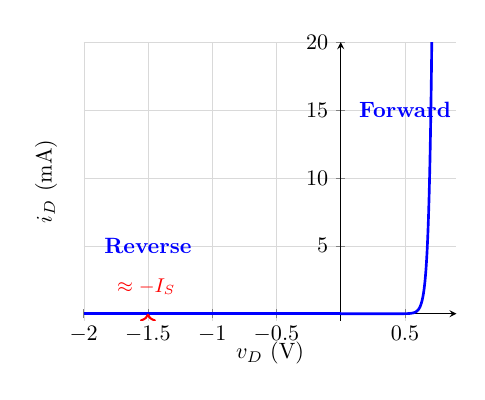
\begin{tikzpicture}[scale=0.8]
            \begin{axis}[
                width=7.5cm, 
                height=6cm,
                xlabel={$v_D$ (V)},
                ylabel={$i_D$ (mA)},
                xmin=-2, 
                xmax=0.9,
                ymin=-0.5, 
                ymax=20,
                grid=major,
                grid style={line width=0.1pt, draw=gray!30},
                axis lines=middle,
                every axis x label/.style={at={(axis description cs:0.5,-0.05)}, anchor=north},
                every axis y label/.style={at={(axis description cs:-0.05,0.5)}, rotate=90, anchor=south},
            ]
            
            % Forward characteristic using Shockley equation
            % Capped to prevent overflow
            \addplot[
                blue, 
                very thick,
                smooth,
                domain=0:0.82,
                samples=150,
                restrict y to domain=0:25
            ] {min(1e-11 * (exp(x/0.025) - 1), 25)};
            
            % Reverse characteristic using Shockley equation
            % For negative voltages, exponential approaches 0
            \addplot[
                blue, 
                very thick,
                smooth,
                domain=-2:0,
                samples=100
            ] {1e-11 * (exp(x/0.025) - 1)};
            
            % Labels
            \node[blue, font=\bfseries] at (axis cs: 0.5,15) {Forward};
            \node[blue, font=\bfseries] at (axis cs:-1.5,5) {Reverse};
            \node[right, red, font=\small] at (axis cs:-1.8,2) {$\approx -I_S$};
            
            % Arrow showing small reverse current
            \draw[red, <->, thick] (axis cs:-1.5,-0.01) -- (axis cs:-1.5,0);
            
            \end{axis}
        \end{tikzpicture}
        \end{center}
        
        \vspace{0.2em}
        One-way current flow
        
    \end{columns}
    
\end{frame}

\section{Small-Signal Resistance}

\begin{frame}{Small-Signal Resistance $r_d$}
    
    \textbf{Two types of resistance}:
    
    \vspace{0.5em}
    
    \begin{columns}[t]
    \column{0.48\textwidth}
        \textbf{DC Resistance}:
        \begin{equation*}
            R_D = \frac{V_D}{I_D}
        \end{equation*}
        
        \begin{itemize}
            \item Total voltage divided by total current
        \end{itemize}
        
        \vspace{0.5em}
        \textbf{Small-Signal Resistance}:
        \begin{equation*}
            r_d = \frac{dv_D}{di_D} = \frac{nV_T}{I_D}
        \end{equation*}
        
        \begin{itemize}
            \item Slope of I-V curve at operating point
            \item Used for small AC signal analysis
            \item Inversely proportional to DC current
        \end{itemize}
    
    \column{0.48\textwidth}
        \textbf{Visualization}:  
        
        \begin{center}
        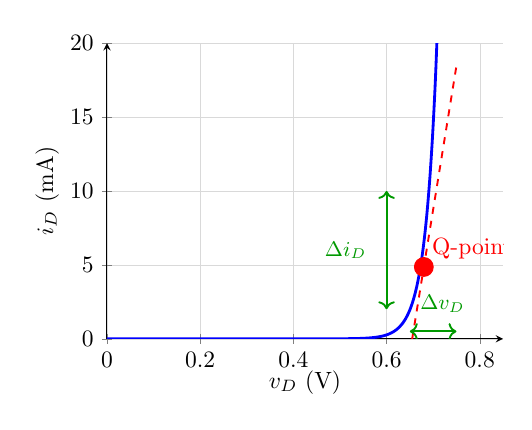
\begin{tikzpicture}[scale=0.85]
            \begin{axis}[
                width=7.5cm, 
                height=6cm,
                xlabel={$v_D$ (V)},
                ylabel={$i_D$ (mA)},
                xmin=0, 
                xmax=0.85,
                ymin=0, 
                ymax=20,
                grid=major,
                grid style={line width=0.1pt, draw=gray!30},
                axis lines=left,
                every axis x label/.style={at={(axis description cs: 0.5,-0.08)}, anchor=north},
                every axis y label/.style={at={(axis description cs:-0.1,0.5)}, rotate=90, anchor=south},
            ]
            
            % I-V curve using Shockley equation
            \addplot[
                blue, 
                very thick,
                smooth,
                domain=0:0.82,
                samples=150,
                restrict y to domain=0:25
            ] {min(1e-11 * (exp(x/0.025) - 1), 25)};
            
            % Operating point at 0.7V (pre-calculated)
            \addplot[only marks, mark=*, red, mark size=4pt] coordinates {(0.68, 4.86)};
            \node[above right, red] at (axis cs:0.68,4.86) {Q-point};
            
            % Tangent line showing r_d
            % Slope at 0.68V ≈ 194.4 mA/V (from derivative)
            % Using equation: y = slope*(x - 0.68) + 4.86
            \addplot[
                red, 
                dashed, 
                thick, 
                domain=0.65:0.75,
                samples=50
            ] {194.4*(x - 0.68) + 4.86};
            
            % Small signal indicators
            \draw[<->, green!60! black, thick] (axis cs: 0.65,0.5) -- (axis cs:0.75,0.5);
            \node[below, green!60! black, font=\small] at (axis cs:0.72,3.5) {$\Delta v_D$};
            
            \draw[<->, green!60!black, thick] (axis cs:0.6,2) -- (axis cs:0.6,10);
            \node[right, green!60!black, font=\small] at (axis cs: 0.45,6) {$\Delta i_D$};
            
            \end{axis}
        \end{tikzpicture}
        \end{center}
        
        Slope at Q-point = $1/r_d$
        
    \end{columns}
    
\end{frame}

\begin{frame}{Calculating Small-Signal Resistance $r_d$}
    
    \begin{columns}[t]
    \column{0.48\textwidth}
        \textbf{Formula}:
        \begin{equation*}
            r_d = \frac{nV_T}{I_D}
        \end{equation*}
        
        At room temperature with $n=1$ and $V_T = 25$ mV:
        \begin{equation*}
            r_d \approx \frac{25 \text{ mV}}{I_D}
        \end{equation*}
        
        \vspace{-0.3cm}
        \textbf{Examples}:
        \begin{center}
             \begin{tabular}{|c|c|}
                \hline
                \textbf{$I_D$} & \textbf{$r_d$} \\
                \hline
                1 mA & 25 $\Omega$ \\
                \hline
                5 mA & 5 $\Omega$ \\
                \hline
                10 mA & 2.5 $\Omega$ \\
                \hline
                100 $\mu$A & 250 $\Omega$ \\
                \hline
            \end{tabular}
        \end{center}

        \vspace{-0.15cm}
        Higher current $\to$ Lower resistance
    
    \column{0.48\textwidth}
        \textbf{Practical Measurement}:
        
        From measurements, use:
        \begin{equation*}
            r_d \approx \frac{\Delta V_D}{\Delta I_D}
        \end{equation*}
        
        \begin{enumerate}
            \item Measure $V_D$ and $I_D$ at operating point
            \item Make small change in $V_D$
            \item Measure new $I_D$
            \item Calculate $r_d$ 
        \end{enumerate}
        
        \textbf{Why It Matters}:
        \begin{itemize}
            \item Essential for AC circuit analysis
            \item Determines circuit impedance
            \item Used in small-signal models
        \end{itemize}
    
    \end{columns}
    
\end{frame}

\section{Zener Diodes}

\begin{frame}{Zener Diodes:   Reverse Breakdown by Design}
    
    \begin{columns}[t]
    \column{0.48\textwidth}
        \textbf{What's Different?   }
        \begin{itemize}
            \item Designed to operate in reverse breakdown
            \item Has a specific breakdown voltage ($V_Z$)
            \item Maintains near constant voltage in breakdown
            \item Used for voltage regulation
        \end{itemize}
        
        \vspace{0.5em}
        \textbf{Symbol}:
        
        \begin{center}
        \begin{circuitikz}[scale=1.5]
            \draw (0,0) to[zD, l=$D_Z$, v=$V_Z$] (2.5,0);
            \node[below] at (0,-0.3) {Anode};
            \node[below] at (2.5,-0.3) {Cathode};
        \end{circuitikz}
        \end{center}
        
        \vspace{0.3em}
        Bent line distinguishes from regular diode
        
    
    \column{0.48\textwidth}
        \textbf{I-V Characteristic}:
        
        \begin{center}
        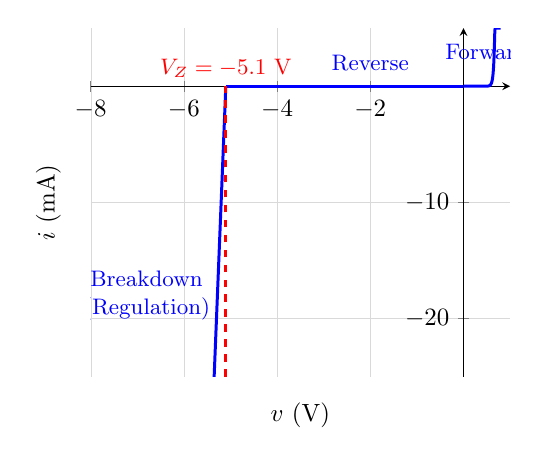
\begin{tikzpicture}[scale=0.9]
            \begin{axis}[
                width=7.5cm, 
                height=6.5cm,
                xlabel={$v$ (V)},
                ylabel={$i$ (mA)},
                xmin=-8, 
                xmax=1,
                ymin=-25, 
                ymax=5,
                grid=major,
                grid style={line width=0.1pt, draw=gray! 30},
                axis lines=middle,
                every axis x label/.style={at={(axis description cs:   0.5,-0.05)}, anchor=north},
                every axis y label/.style={at={(axis description cs:-0.05,0.5)}, rotate=90, anchor=south},
            ]
            
            % Forward region using Shockley equation 
            \addplot[
                blue, 
                very thick,
                smooth,
                domain=0:0.8,
                samples=100,
                restrict y to domain=0:5
            ] {min(1e-11 * (exp(x/0.025) - 1), 5)};
            
            % Reverse region before breakdown (negative voltage, small negative current)
            \addplot[
                blue, 
                very thick,
                smooth,
                domain=-5.1:0,
                samples=50
            ] {1e-11 * (exp(x/0.025) - 1)};
            
            % Breakdown region 
            \addplot[
                blue, 
                very thick,
                smooth,
                domain=-7.5:-5.1,
                samples=100
            ] {100*(x + 5.1) - 0.01};
            
            % Highlight breakdown voltage
            \draw[red, dashed, very thick] (axis cs:-5.1,-25) -- (axis cs:-5.1,0);
            \node[red, above, font=\small] at (axis cs:-5.1,0) {$V_Z = -5.1$ V};
            
            % Labels
            \node[blue, font=\small] at (axis cs:0.5,3) {Forward};
            \node[blue, font=\small] at (axis cs:-2,2) {Reverse};
            \node[blue, font=\small, align=center] at (axis cs:-6.8,-18) {Breakdown \\ (Regulation)};
            
            \end{axis}
        \end{tikzpicture}
        \end{center}
        
        Voltage stays near $V_Z$ as current varies
        
    \end{columns}
    
\end{frame}

\begin{frame}{Zener Voltage Regulation}
    
    \begin{columns}[t]
    \column{0.48\textwidth}
        \textbf{Simple Voltage Regulator}:

        \vspace{-0.5cm}
        
        \begin{center}
        \begin{circuitikz}[scale=0.8]
            \draw (0,0) to[V, l=$V_{in}$, invert] (0,3)
                  to[R, l=$R$, i=$I$] (3,3)
                  to[short, -*] (3,3);
            \draw (3,3) to[zD, l=$D_Z$, v=$V_Z$, invert] (3,0)
                  to[short] (0,0);
            \draw (3,3) to[short, i=$I_L$] (6,3)
                  to[R, l_=$R_L$, v^=$V_{out}$] (6,0)
                  to[short] (3,0);
            \node[ground] at (1.5,0) {};
        \end{circuitikz}
        \end{center}
        
        \vspace{-0.5cm}
        \textbf{Operation}:
        \begin{itemize}
            \item $V_{in}$ must be greater than $V_Z$
            \item Zener maintains $V_{out} \approx V_Z$
            \item Works even if $V_{in}$ or $I_L$ varies
            \item Series resistor $R$ limits current
        \end{itemize}
    
    \column{0.48\textwidth}
        \textbf{Zener Model in Breakdown}:
        
        \begin{center}
        \begin{circuitikz}[scale=0.8]
            \draw (0,0) to[battery1, l=$V_Z$] (2,0)
                  to[R, l=$r_z$] (4,0);
            \draw[dashed] (-0.5,-0.8) rectangle (4.5,1.1);
            \node at (2,-1.3) {Zener model};
        \end{circuitikz}
        \end{center}

        \vspace{-0.8cm}
        
        \begin{equation*}
            V_{actual} = V_Z + r_z \cdot I_Z
        \end{equation*}
        
        \vspace{0.3em}
        \textbf{Small-Signal Resistance} ($r_z$):
        \begin{itemize}
            \item Smaller $r_z$ = better regulation
            \item Measure as $r_z = \Delta V_Z / \Delta I_Z$
        \end{itemize}
        
        \vspace{0.3em}
        \begin{block}{Important}
            $P_Z = V_Z \times I_Z$ must be within power rating
        \end{block}
    
    \end{columns}
    
\end{frame}

\section{Lab Preview}

\begin{frame}{What You'll Do in Lab}
    
    \begin{columns}[t]
    \column{0.48\textwidth}
        \textbf{Experiment 1: Forward Bias}
        \begin{itemize}
            \item Measure I-V characteristics
            \item Observe exponential behavior
            \item Identify turn-on voltage
        \end{itemize}
        
        \vspace{0.5em}
        \textbf{Experiment 2: Small-Signal Resistance}
        \begin{itemize}
            \item Calculate $r_d$ from measurements
            \item Verify theoretical predictions
            \item Compare at different operating points
            \item Understand slope of I-V curve
        \end{itemize}
    
    \column{0.48\textwidth}
        \textbf{Experiment 3: Reverse Bias}
        \begin{itemize}
            \item Measure reverse current
            \item Verify saturation current behavior
            \item Understand one-way conduction
        \end{itemize}

        \vspace{0.5em}
        \textbf{Experiment 4-5: Zener Diodes}
        \begin{itemize}
            \item Measure breakdown characteristics
            \item Determine Zener voltage
            \item Calculate Zener resistance $r_z$
            \item Verify voltage regulation
        \end{itemize}
        

    \end{columns}
    
\end{frame}

\section{Summary}

\begin{frame}{Summary: Diode Fundamentals}
    
    \begin{columns}[t]
    \column{0.48\textwidth}
        \textbf{Key Concepts}:
        \begin{itemize}
            \item Diodes are one-way current devices
            \item Forward bias: conducts at $\approx 0.7$ V
            \item Reverse bias: blocks current ($\approx -I_S$)
            \item Exponential I-V relationship
        \end{itemize}
        
        \vspace{0.5em}
        \textbf{Important Equations}:
        \begin{itemize}
            \item Shockley: $i_D = I_S(e^{v_D/nV_T} - 1)$
            \item Small-signal: $r_d = nV_T/I_D$
            \item Thermal voltage: $V_T \approx 25$ mV
        \end{itemize}
        
    \column{0.48\textwidth}
        \textbf{Zener Diodes}:
        \begin{itemize}
            \item Operate in reverse breakdown
            \item Maintain constant voltage $V_Z$
            \item Used for voltage regulation
            \item Model: $V_Z$ + small resistance $r_z$
        \end{itemize}
        
        \vspace{0.5em}
        \textbf{Next Topics}:
        \begin{itemize}
            \item Diode circuit analysis
            \item Rectifier circuits (AC to DC)
            \item Bridge rectifiers
        \end{itemize}
        
    \end{columns}
    
    \vspace{1em}
    
    \begin{block}{Prepare for Lab}
        Review Shockley equation, understand forward/reverse bias, and complete pre-lab questions
    \end{block}
    
\end{frame}

\end{document}
